\documentclass[12pt]{article}
\usepackage{bookmark}
\usepackage{minted,xcolor}
\usepackage{graphicx}
\usepackage{hyperref}
\usepackage{geometry}
\usepackage{circuitikz}
\usepackage{wrapfig}
\usepackage{amsmath}
\usepackage{amssymb}
\usepackage[utf8]{inputenc}
\usepackage[export]{adjustbox}
\newcommand{\Sum} [2] {\the\numexpr #1 + #2 \relax \\}
\definecolor{mygray}{RGB}{238, 238, 238}
% \definecolor{bg}{RGB}{40,42,54}
\definecolor{bg}{RGB}{46, 46, 46}
\graphicspath{ {images/} }
\hypersetup{
    colorlinks=true,
    linkcolor=blue,
    filecolor=magenta,      
    urlcolor=orange,
}
\urlstyle{same}
\geometry{a4paper, margin=1in}
\usemintedstyle{monokai}
\title{ELP201 Lab Report}
\author{Adit Malhotra}
\date{2020EE10458}
\begin{document}
\maketitle
\tikzstyle{branch}=[fill,shape=circle,minimum size=3pt,inner sep=0pt]
\section{Truth Table}
Given function $\rightarrow F= \sum(0,1,2,5,6,8,9,11,13,14,15)$
\begin{center}
    \begin{tabular}{||c c c c c c||} 
     \hline
     A & B & C & D & Output (F) & Minterm\\ [0.5ex] 
     \hline
     \hline
     0 & 0 & 0 & 0 & 1 & $m_{0}$\\ 
     \hline
     0 & 0 & 0 & 1 & 1 & $m_{1}$\\ 
     \hline
     0 & 0 & 1 & 0 & 1 & $m_{2}$\\ 
     \hline
     0 & 0 & 1 & 1 & 0 & $m_{3}$\\ 
     \hline
     0 & 1 & 0 & 0 & 0 & $m_{4}$\\ 
     \hline
     0 & 1 & 0 & 1 & 1 & $m_{5}$\\
     \hline
     0 & 1 & 1 & 0 & 1 & $m_{6}$\\
     \hline
     0 & 1 & 1 & 1 & 0 & $m_{7}$\\
     \hline
     1 & 0 & 0 & 0 & 1 & $m_{8}$\\ 
     \hline
     1 & 0 & 0 & 1 & 1 & $m_{9}$\\ 
     \hline
     1 & 0 & 1 & 0 & 0 & $m_{10}$\\ 
     \hline
     1 & 0 & 1 & 1 & 1 & $m_{11}$\\ 
     \hline
     1 & 1 & 0 & 0 & 0 & $m_{12}$\\ 
     \hline
     1 & 1 & 0 & 1 & 1 & $m_{13}$\\ 
     \hline
     1 & 1 & 1 & 0 & 1 & $m_{14}$\\ 
     \hline
     1 & 1 & 1 & 1 & 1 & $m_{15}$\\ [1ex] 
     \hline
    \end{tabular}
    \end{center}
\section{Implementation of the function}
\subsection{Using one 8x1 MUX}
Since there are three selection lines availabe for the 8x1 MUX, thus three of the input variables $(B,C,D)$ can be used as selection lines of the MUX. Now depending on the type of minterms in the function, A, $\bar{A}$, 1, 0 will be used as appropriate input lines to the MUX. Exact circuit diagram is given below:
\begin{figure}[H]
\centering
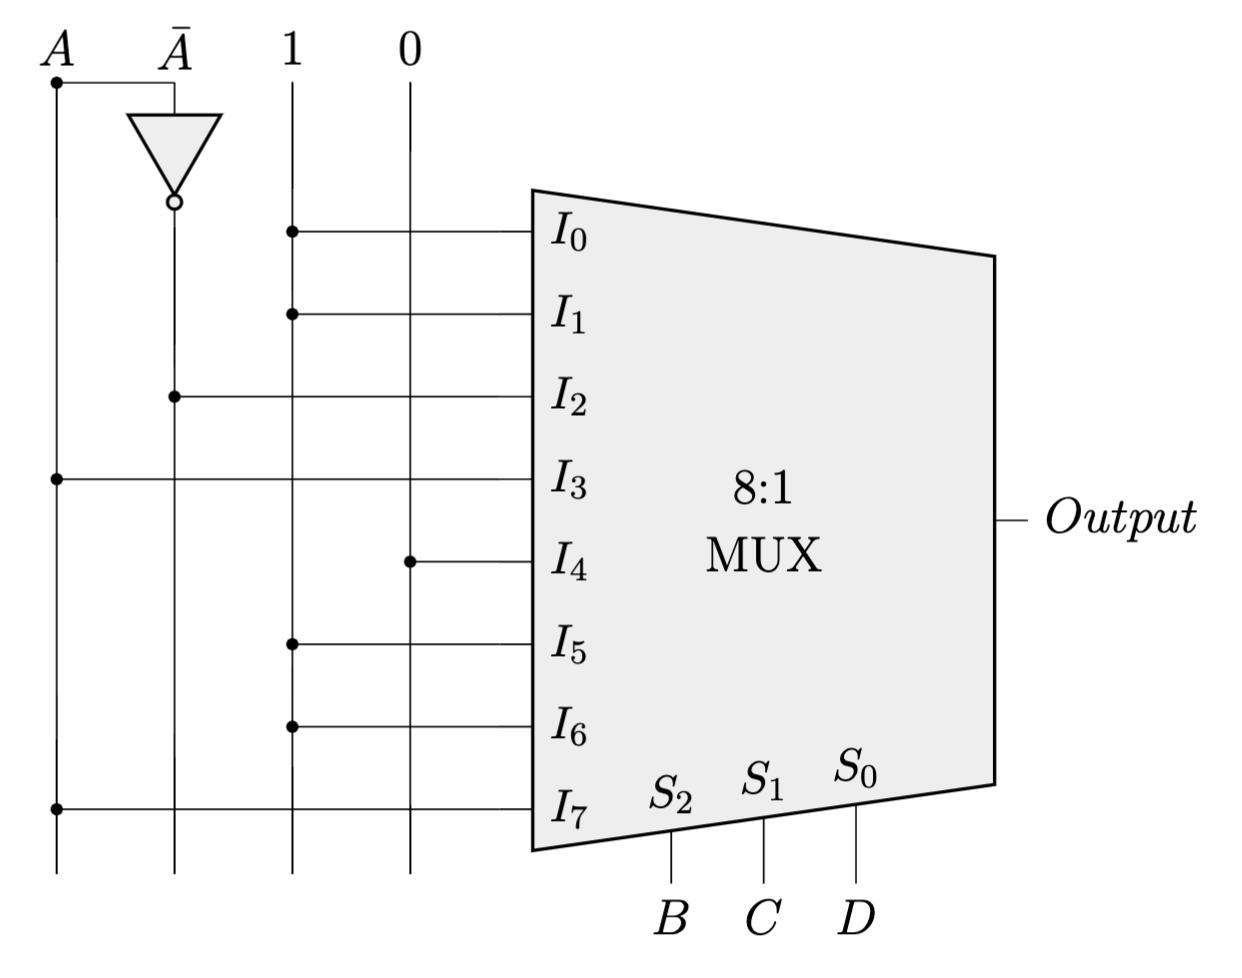
\includegraphics[width=0.6\textwidth]{8x1.png}
\caption{Realisation of the function using a $8\times1 \ MUX$}
\end{figure}
\subsection{Using two 4x1 MUX}
In case of two 4:1 multiplexers, two of the input variables (D and C) will be used as selection lines of the two joint multiplexers, and one variable can be used as $Enable\ Line$ with direct line to one of the mux and with a NOT gate to other mux, so that only one of the mux is active at a moment. Finally the OR of the outputs from the muxes would result in output. In this way we have combined two 4:1 muxes into a single 8:1 mux.
\begin{figure}[H]
    \centering
    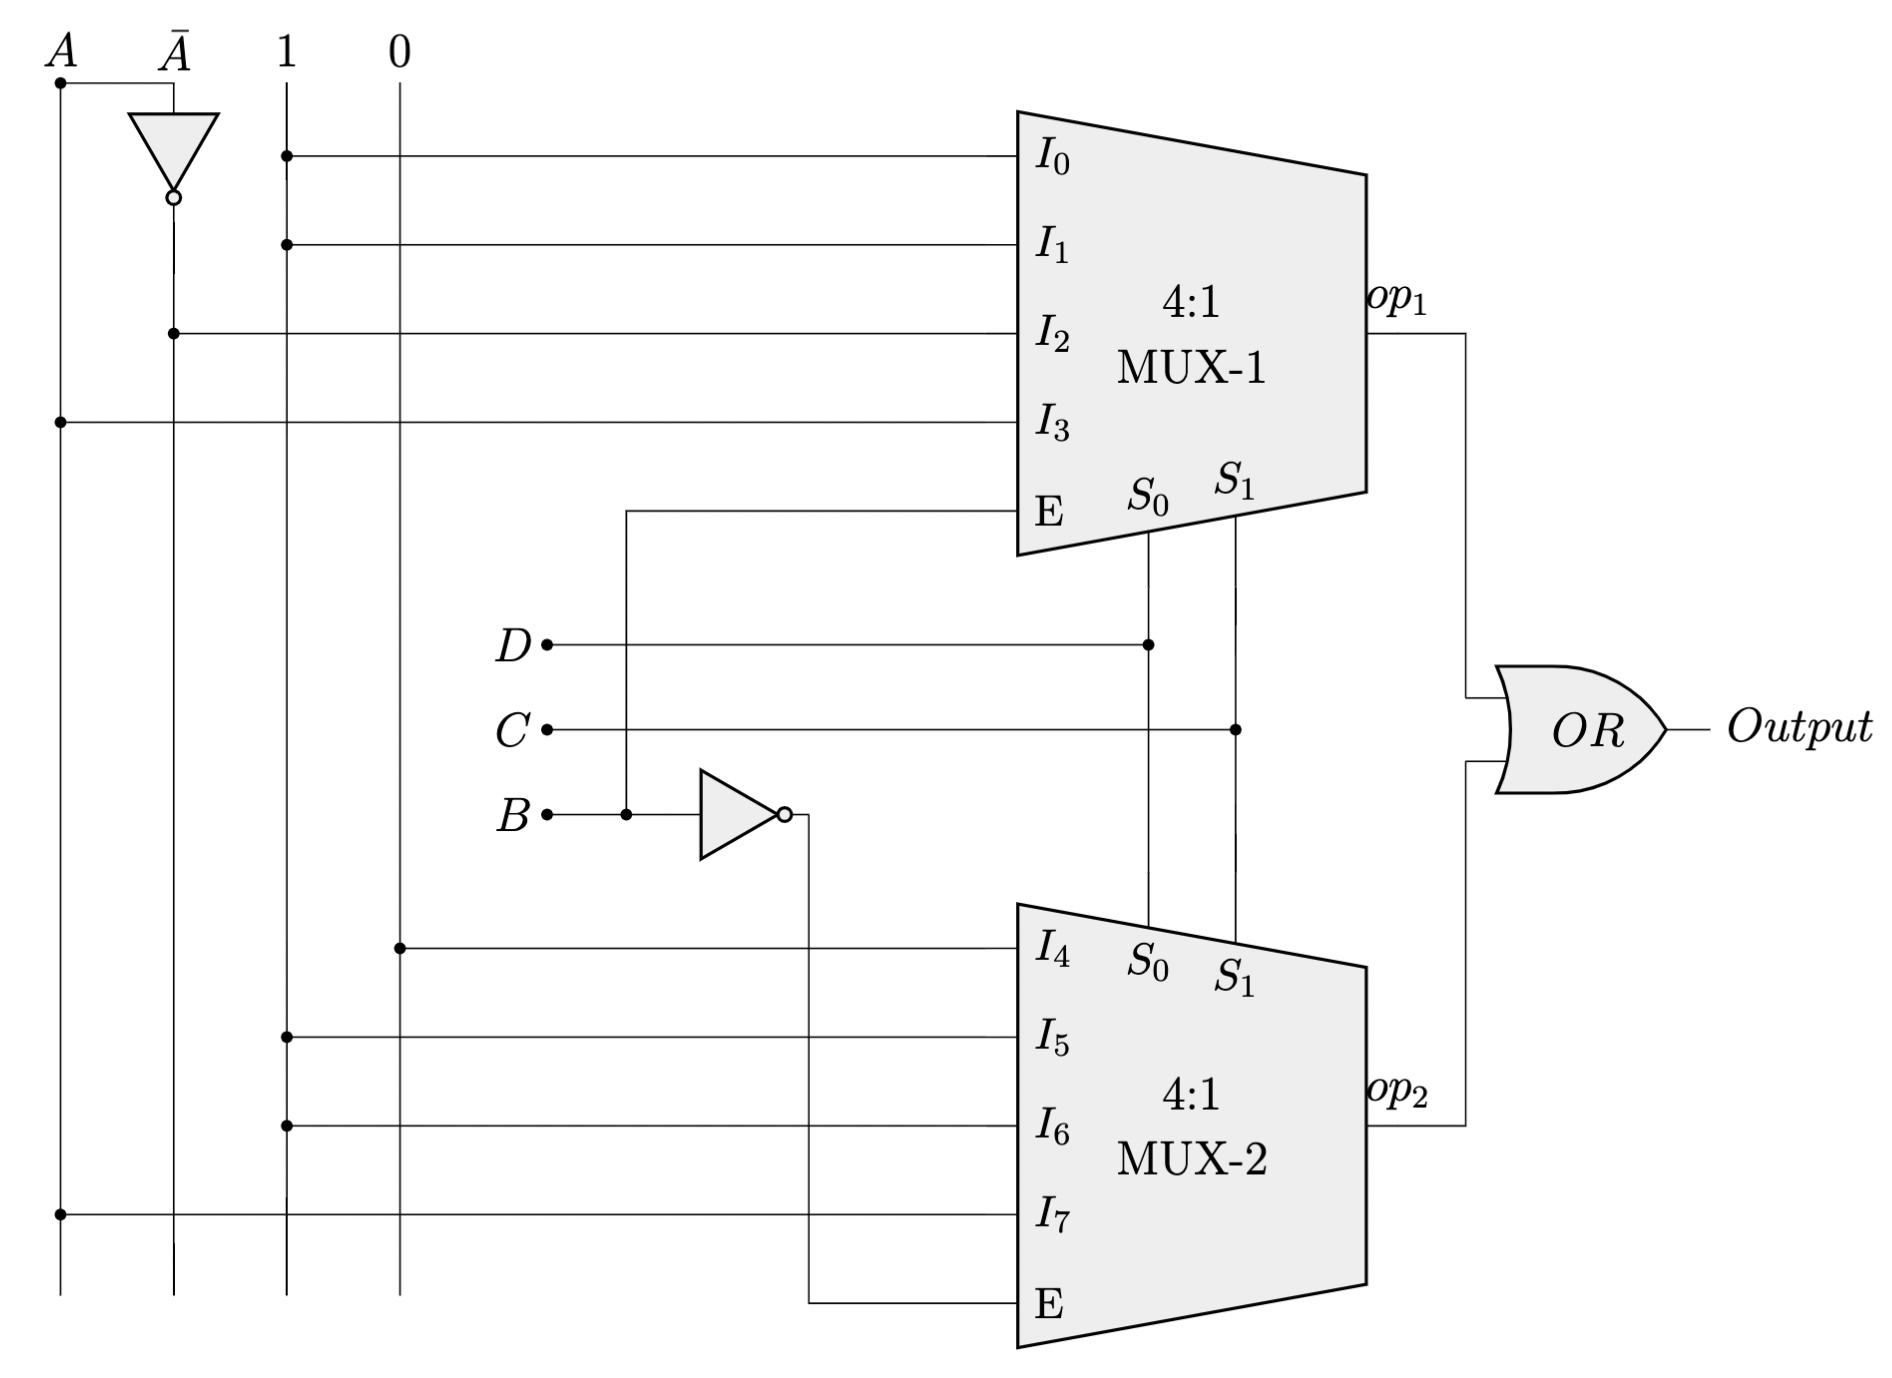
\includegraphics[width=0.85\textwidth,right]{4x1.png}
    \caption{Realisation of the function using two $4\times1 \ MUX$}
    \end{figure}
\section{Verilog part}
\subsection{Simplification using K-Maps}
\begin{wrapfigure}{R}{0.7\textwidth}
    \begin{center}
      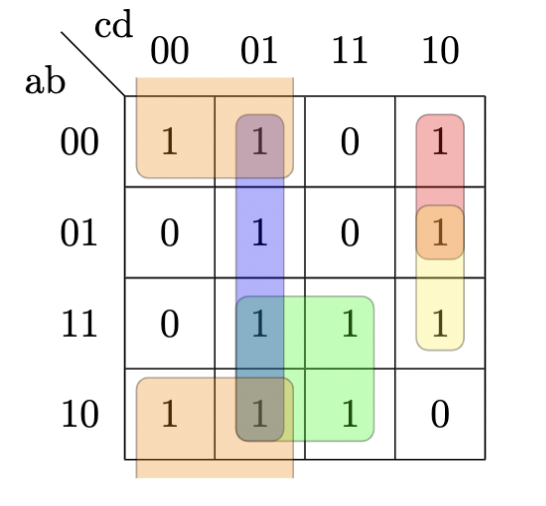
\includegraphics[width=0.3\textwidth]{k-map.png}
    \end{center}
    \caption{K-Map for the function}
  \end{wrapfigure}
  By marking the minterms on the K-Map, the \\implicants come out to be $AD,\ \bar{B}\bar{C},\ \bar{C}D,\ \bar{A}C\bar{D},\ BC\bar{D}$.\\
  \\ Thus the simplified \\expression for F is:
  $$F = AD\ +\ \bar{B}\bar{C}\ +\ \bar{C}D\ +\ \bar{A}C\bar{D}\ +\ BC\bar{D}$$
\\ \\ \\
\subsection{Code}
The code for file containing the implementation of $8\times1\ mux$, $4\times1\ mux$ and realisation of the function using k-maps (design.v) : 
\inputminted[bgcolor=bg,frame=lines,framesep=2mm,numbers=left]
{Verilog}{./code_files/design.v}
\\ \\ \\
The code for the testbench file (main.v), the wire $y1$ is the output obtained when the function is realised using only $8\times1\ mux$, the wire $y2$ is the output obtained when the function is realised using two $4\times1\ mux$ and finally wire $F$ is output of the function when realised using kmaps  :
\inputminted[bgcolor=bg,frame=lines,framesep=2mm,numbers=left]
{Verilog}{./code_files/main.v}
\\ \\ \\ \\ \\
\subsection{The waveform output}
Thus it can be observed that output of $y1$ and $y2$ is exactly same as $F$, hence we have correctly implemented the function using the multiplexers in both the cases.
\begin{figure}[H]
  \centering
  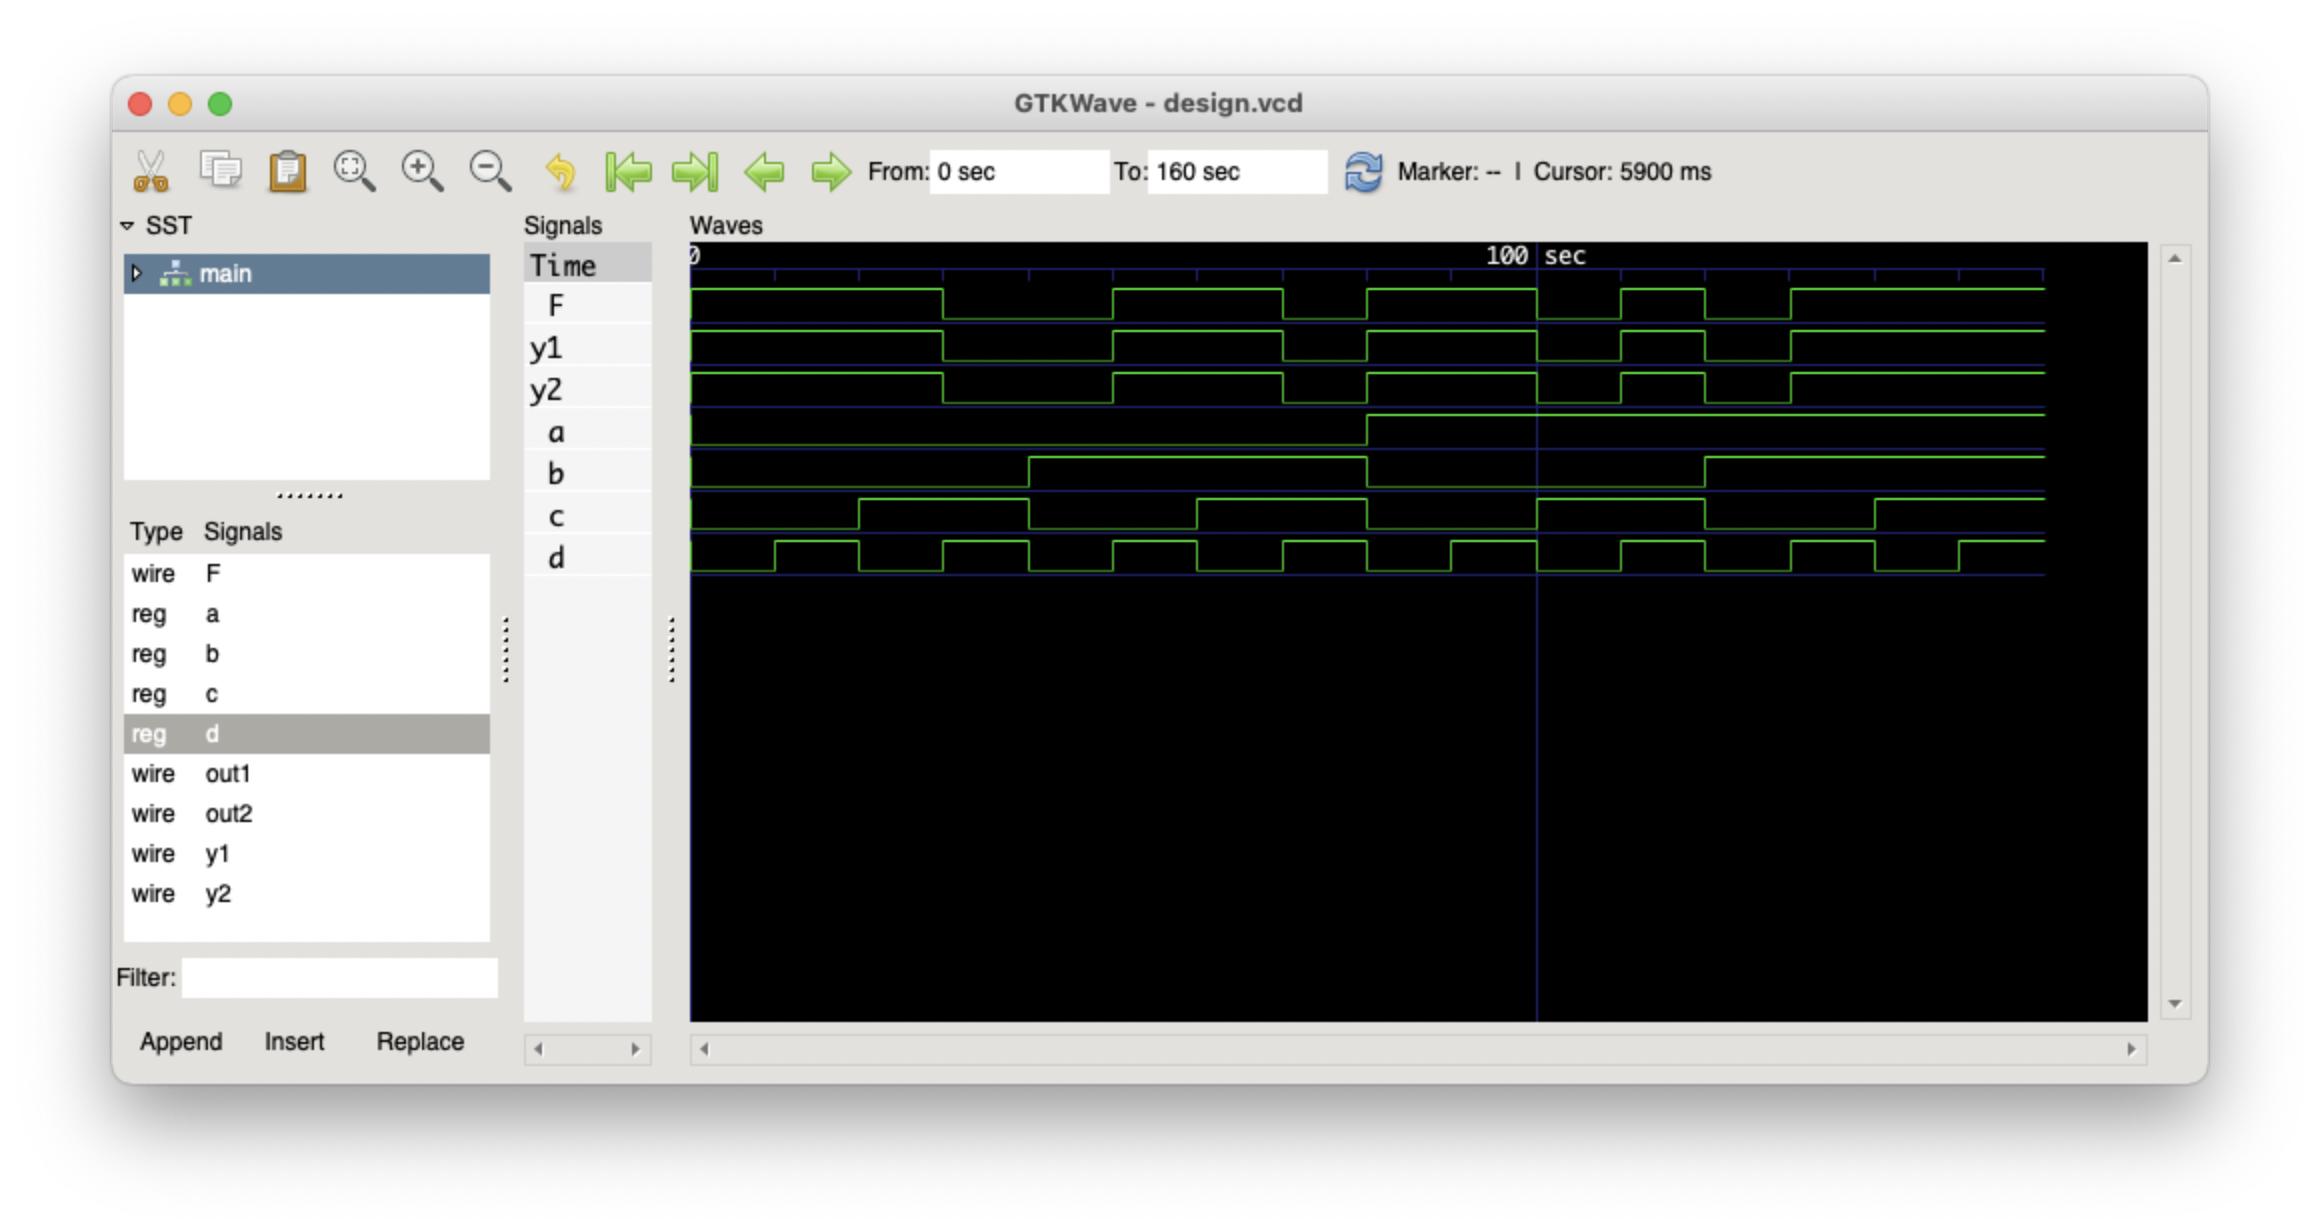
\includegraphics[width=1\textwidth]{plot.png}
  % \caption{Realisation of the function using two $4\times1 \ MUX$}
  \end{figure}
The code files can be downloaded from \href{https://drive.google.com/uc?export=download&id=1I1zmg8S1jMNQBCqtZEEszLOsPr9Juvdl}{\textbf{here}}.
\end{document}


% \begin{circuitikz}
%     \ctikzset{logic ports=ieee}
%     \node (x3) at (0,-1.5) {$A$};
%     \node (x2) at (1,-1.5) {$ \bar{A} $};
%     \node (x1) at (2,-1.5) {$1$};
%     \node (x0) at (3,-1.5) {$0$};
%     \node (x4) at (4,-6.75) {$D$};
%     \node (x5) at (4,-7.5) {$C$};
%     \node (x6) at (4,-8.25) {$B$};

%     \ctikzset{logic ports/fill=mygray}
%     \ctikzset{logic ports/scale=0.7}
%     \node[not port , draw, rotate=-90] at ($(x3)+(1,-0.9)$) (Not3) {};
%     \node[not port , draw] at ($(x6)+(2,0)$) (Not6) {};
%     \ctikzset{logic ports/scale=1}
%     \node[or port , draw] at (13.5,-7.5) (or1) {$OR$};
%     \node[right] at (or1.out) {$Output$};
%     \foreach \i in {3}
%     {
%         \path (x\i) -- coordinate (punt\i) (x\i |- Not\i.in 1);
%         \draw (punt\i) node[branch] {} -| (Not\i.in 1);
%     }

%     \node [muxdemux, muxdemux def={NL=5,NB=4,NR=1,w=5.5,Lh=7,Rh=5,square pins=1},draw only bottom pins={2-3},fill=mygray](mux1) at(10,-4){};
%     \node[above] at (mux1.center) {4:1};
%     \node[below] at (mux1.center) {MUX-1};
%     \node[above] (opt1) at (mux1.rpin 1) {$op_{1}$};
%     \node[right,font=\small] at (mux1.blpin 5) {E};

%     \foreach \myp in {1,2,3,4} 
%         \node[right, font=\small] at (mux1.blpin \myp) {$I_{\Sum {-1} {\myp}}$};
%     \foreach \myp in {2,3} 
%         \node[above,font=\small] at (mux1.bbpin \myp) {$S_{\Sum {-2} {\myp}}$};
    
%     \node [muxdemux, muxdemux def={NL=5,NB=0,NT=4,NR=1,w=5.5,Lh=7,Rh=5,square pins=1},draw only top pins={2-3},fill=mygray](mux2) at(10,-11){};
%     \node[above] at (mux2.center) {4:1};
%     \node[below] at (mux2.center) {MUX-2};
%     \node[above] (opt2) at (mux2.rpin 1) {$op_{2}$};
%     \node[right,font=\small] at (mux2.blpin 5) {E};
    
%     \foreach \myp in {1,2,3,4} 
%         \node[right, font=\small] at (mux2.blpin \myp) {$I_{\Sum {3} {\myp}}$};
%     \foreach \myp in {2,3} 
%         \node[below,font=\small] at (mux2.btpin \myp) {$S_{\Sum {-2} {\myp}}$};
    
%     \draw (x3) |- (0,-12.5);
%     \draw (Not3.out) |- (1,-12.5);
%     \draw (x1) |- (2,-12.5);
%     \draw (x0) |- (3,-12.5);

%     \draw (mux1.bpin 2) |- (mux2.tpin 2);
%     \draw (mux1.bpin 3) |- (mux2.tpin 3);
%     \draw ($(x6)+(0.3,0)$) node[branch]{} |- (Not6.in 1);
%     \draw ($(x5)+(0.3,0)$) node[branch] {} |- (mux1.bpin 3 |- x5) node[branch] {};
%     \draw ($(x4)+(0.3,0)$) node[branch] {} |- (mux1.bpin 2 |- x4) node[branch] {};
%     \draw (Not6.out) |- (mux2.lpin 5);
%     \draw ($(x6)+(1,0)$) node[branch] {} |- (mux1.lpin 5);

%     \draw (x3 |- mux1.lpin 4) node[branch] {} -- (mux1.lpin 4);
%     \draw (x3 |- mux2.lpin 4) node[branch] {} -- (mux2.lpin 4);
%     \draw (x2 |- mux1.lpin 3) node[branch] {} -- (mux1.lpin 3);
%     \draw (x1 |- mux1.lpin 1) node[branch] {} -- (mux1.lpin 1);
%     \draw (x1 |- mux1.lpin 2) node[branch] {} -- (mux1.lpin 2);
%     \draw (x1 |- mux2.lpin 2) node[branch] {} -- (mux2.lpin 2);
%     \draw (x1 |- mux2.lpin 3) node[branch] {} -- (mux2.lpin 3);
%     \draw (x0 |- mux2.lpin 1) node[branch] {} -- (mux2.lpin 1);
%     \draw (mux1.rpin 1) -| (or1.in 1);
%     \draw (mux2.rpin 1) -| (or1.in 2);

% \end{circuitikz}





% \begin{circuitikz}
%     \ctikzset{logic ports=ieee}
%     \node (x3) at (0,0) {$A$};
%     \node (x2) at (1,0) {$ \bar{A} $};
%     \node (x1) at (2,0) {$1$};
%     \node (x0) at (3,0) {$0$};

%     \ctikzset{logic ports/fill=mygray}
%     \ctikzset{logic ports/scale=0.7}
%     \node[not port , draw, rotate=-90] at ($(x3)+(1,-0.9)$) (Not3) {};
%     \foreach \i in {3}
%     {
%         \path (x\i) -- coordinate (punt\i) (x\i |- Not\i.in 1);
%         \draw (punt\i) node[branch] {} -| (Not\i.in 1);
%     }

%     \node [muxdemux, muxdemux def={NL=8,NB=5,NR=1,w=7,Lh=10,Rh=8, inset Rh=1.0,inset w=1,square pins=1},draw only bottom pins={2-4},fill=mygray](mux1) at(6,-4){};
%     \node[above] at (mux1.center) {8:1};
%     \node[below] at (mux1.center) {MUX};
%     \node[below] (y3) at (mux1.bpin 2) {$B$};
%     \node[below] (y2) at (mux1.bpin 3) {$C$};
%     \node[below] (y1) at (mux1.bpin 4) {$D$};
%     \node[right] (opt) at (mux1.rpin 1) {$Output$};

%     \foreach \myp in {1,2,3,4,5,6,7,8} 
%         \node[right, font=\small] at (mux1.blpin \myp) {$I_{\Sum {-1} {\myp}}$};
%     \foreach \myp in {2,3,4} 
%         \node[above,font=\small] at (mux1.bbpin \myp) {$S_{\Sum {4} {-\myp}}$};
    
%     \draw (x3) |- (0,-7);
%     \draw (Not3.out) |- (1,-7);
%     \draw (x1) |- (2,-7);
%     \draw (x0) |- (3,-7);

%     \draw (x1 |- mux1.lpin 1) node[branch] {} -- (mux1.lpin 1);
%     \draw (x1 |- mux1.lpin 2) node[branch] {} -- (mux1.lpin 2);
%     \draw (x2 |- mux1.lpin 3) node[branch] {} -- (mux1.lpin 3);
%     \draw (x3 |- mux1.lpin 4) node[branch] {} -- (mux1.lpin 4);
%     \draw (x0 |- mux1.lpin 5) node[branch] {} -- (mux1.lpin 5);
%     \draw (x1 |- mux1.lpin 6) node[branch] {} -- (mux1.lpin 6);
%     \draw (x1 |- mux1.lpin 7) node[branch] {} -- (mux1.lpin 7);
%     \draw (x3 |- mux1.lpin 8) node[branch] {} -- (mux1.lpin 8);
% \end{circuitikz}